\documentclass{amsart}

\usepackage[english]{babel}
\usepackage[utf8]{inputenc}
\usepackage{graphicx}
\usepackage{mathtools}
\usepackage{amsthm}
\usepackage{thmtools,thm-restate}
\usepackage{amsfonts}
\usepackage{hyperref}
\usepackage[backend=biber,url=true,doi=true,eprint=false,style=alphabetic]{biblatex}
\usepackage{enumitem}
\usepackage[justification=centering,singlelinecheck=false]{caption}
\usepackage{indentfirst}
\usepackage{algorithm}
\usepackage{algpseudocode}
\usepackage{listings}
\usepackage[x11names, rgb]{xcolor}
\usepackage{tikz}
\usepackage{hyperref}
\usepackage{subcaption}
\usepackage{booktabs}
\usepackage{linegoal}
\usepackage{csquotes}
\usetikzlibrary{snakes,arrows,shapes}

\addbibresource{references.bib}

\makeatletter
\def\subsection{\@startsection{subsection}{3}%
  \z@{.5\linespacing\@plus.7\linespacing}{.1\linespacing}%
  {\normalfont}}
\makeatother

\makeatletter
\patchcmd{\@setauthors}{\MakeUppercase}{}{}{}
\makeatother

\DeclareMathOperator*{\argmin}{arg\,min}
\DeclareMathOperator*{\argmax}{arg\,max}
\DeclareMathOperator*{\Val}{\text{Val}}
\DeclareMathOperator*{\Ch}{\text{Ch}}
\DeclareMathOperator*{\Pa}{\text{Pa}}
\DeclareMathOperator*{\Sc}{\text{Sc}}
\newcommand{\ov}{\overline}

\newcommand\defeq{\mathrel{\overset{\makebox[0pt]{\mbox{\normalfont\tiny\sffamily def}}}{=}}}

\newcommand{\algorithmautorefname}{Algorithm}
\algrenewcommand\algorithmicrequire{\textbf{Input}}
\algrenewcommand\algorithmicensure{\textbf{Output}}
\algnewcommand{\LineComment}[1]{\State\,\(\triangleright\) #1}

\captionsetup[table]{labelsep=space}

\theoremstyle{plain}

\newcounter{dummy-def}\numberwithin{dummy-def}{section}
\newtheorem{definition}[dummy-def]{Definition}
\newcounter{dummy-thm}\numberwithin{dummy-thm}{section}
\newtheorem{theorem}[dummy-thm]{Theorem}
\newcounter{dummy-prop}\numberwithin{dummy-prop}{section}
\newtheorem{proposition}[dummy-prop]{Proposition}
\newcounter{dummy-corollary}\numberwithin{dummy-corollary}{section}
\newtheorem{corollary}[dummy-corollary]{Corollary}
\newcounter{dummy-lemma}\numberwithin{dummy-lemma}{section}
\newtheorem{lemma}[dummy-lemma]{Lemma}
\newcounter{dummy-ex}\numberwithin{dummy-ex}{section}
\newtheorem{exercise}[dummy-ex]{Exercise}
\newcounter{dummy-eg}\numberwithin{dummy-eg}{section}
\newtheorem{example}[dummy-eg]{Example}

\numberwithin{equation}{section}

\newcommand{\set}[1]{\mathbf{#1}}
\newcommand{\pr}{\mathbb{P}}
\newcommand{\eps}{\varepsilon}
\renewcommand{\implies}{\Rightarrow}

\newcommand{\bigo}{\mathcal{O}}

\setlength{\parskip}{1em}

\lstset{frameround=fttt,
	numbers=left,
	breaklines=true,
	keywordstyle=\bfseries,
	basicstyle=\ttfamily,
}

\newcommand{\code}[1]{\lstinline[mathescape=true]{#1}}
\newcommand{\mcode}[1]{\lstinline[mathescape]!#1!}
\newcommand{\dset}[1]{\mathcal{#1}}

\title{%
  \noindent\rule{13cm}{1.0pt}\\
  \vspace{0.2cm}
  The Poon-Domingos Parameter Learning Algorithm for Image Completion and Classification on
  Sum-Product Networks
  \noindent\rule{13cm}{0.8pt}
}
\xdef\shorttitle{The Poon-Domingos Algorithm}
\author[]{\normalsize\textbf{Renato Lui Geh}\\\small Computer Science\\Institute of Mathematics
  and Statistics\\University of São Paulo\\\texttt{renatolg@ime.usp.br}}

\begin{document}

\begin{abstract}
  In this document we describe the Poon-Domingos~\cite{poon-domingos} parameter learning algorithm
  for image classification and completion.
  \vspace*{-3.5em}
\end{abstract}

\maketitle

\section{Structure}

The Poon-Domingos algorithm uses a fixed structure and then learns the weights through generative
learning. We first give an overview on how to build the structure given an image and then provide a
pseudo-code algorithm for building such structure.

\subsection{Overview}

The Poon architecture models a probability distribution over a set of images. It is constructed by
taking all possible rectangular axis-aligned regions in the image and assigning product nodes to
each of these regions. Two sum nodes are then added as children for each of these regions,
representing all the possible pairings of subregions in each region determined by the axis-aligned
division set in the previous step. We then add the product nodes to a single sum node that
represents the undivided original area. We then recursively apply the same steps on each sum node
we constructed this way, taking that sum node as the new root of the sub-SPN\@. The Poon structure
accepts different multiple resolution levels. At every region splitting, we consider a step $r$
that indicates how fine the granularity is for the architecture.

\begin{figure}[h]
  \centering
  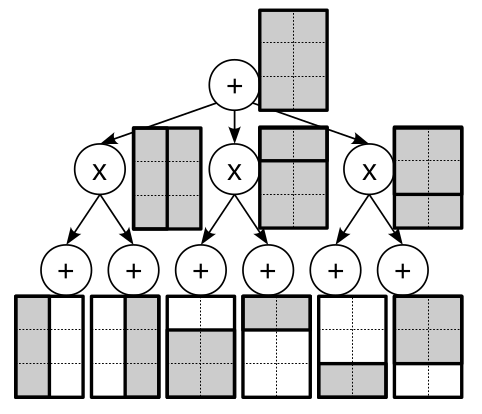
\includegraphics[scale=1.0]{imgs/dv_spn.png}
  \captionsetup{justification=raggedright}
  \caption{The Poon architecture with $r = 1$ resolution. At each product node division, we
  consider an $r$ length division on each axis. Since $r=1$ in this case, we have $3$ product
  nodes, with each of their two possible subregions represented by sum nodes. Note how product
  nodes are always decomposable and sum nodes are always complete.\label{fig:dv_spn}}
\end{figure}

\subsection{Definitions and properties}

Let us organize in a clearer way what we have extracted from~\cite{clustering}.

\begin{definition}[Region] A region $\pi$ is a product node. Graphically, it represents an
  axis-aligned rectangular region of the image. We shall denote an SPN $S(\cdot)$ rooted at a
  region as $\pi(\cdot)$.
\end{definition}

\begin{definition}[Subregion] A subregion $\sigma$ is a sum node. Given a region $R$, the children
  of $R$ are the two possible rectangles that compose $R$. We shall denote an SPN rooted at a
  subregion as $\sigma(\cdot)$.
\end{definition}

The idea behind the Poon structure algorithm is to recursively take a rectangular subarea of an
image and divide it into all $k$ possible regions given a granularity $r$, with each region having
two children (subregions) that represent the possible pairings of each region. We then recurse
through each of these subregions.

Let $I (x_0, y_0, x_1, y_1)$ be the area of the image we are to create the structure for, with
$ (x_0, y_0)$ and $ (x_1, y_1)$ being the top left and bottom right positions in the image. The
entire image is given by $I (0, 0, w, h)$, where $w, h$ are the width and height of the image
respectively.

A subregion $\sigma$ implicitly represents an area $I (x_0, y_0, x_1, y_1)$, whilst each region of
$\sigma$ is a possible subdivision of $I$ by drawing a line, either horizontally or vertically,
through one of the axis of $I$, partitioning it into two subregions.

We can clearly see that, for a subregion $\sigma$, there are $x_1-x_0$ possible vertically divided
regions and $y_1-y_0$ horizontally divided regions, bringing the total to $ (x_1+y_1)- (x_0+y_0)$
possible product nodes as children of $\sigma$ for $r=1$. For the general case, we can clearly see
that we have $\lceil (x_1-x_0)/r\rceil + \lceil (y_1-y_0)/r\rceil$ possible regions.

%\begin{proposition} The height of a Poon-Domingos SPN structure is $2w+2h-3$.
%\end{proposition}
%\begin{proof}
  %Let $h$ be the height of an SPN $S$. Maximizing $h$ is finding the longest path $p$ from a leaf
  %(in this case the image's pixel) to the root node. Let us assume $(x, y)$ as the farthest leaf's
  %pixel representation from the root node. Since a region cuts an area $I$ either horizontally or
  %vertically, with each subregion being the two possible subregions, we can easily see that in
  %order to maximize $p$ we must maximize the number
%\end{proof}

\subsection{Algorithm}

The structure algorithm is recursive. It takes as parameters a sum node $S$ as root of the SPN, the
$ (x_0,y_0)$ top-left position of the subregion $S$ relative to the original complete image, the
$ (x_1,y_1)$ bottom-right position of the subregion $S$, the resolution granularity step $k$ and a
dataset $\dset{D}$ where $\dset{D}[X]$ is the set of instances of variable $X$.

Let's define a few helper functions before we see the algorithm. Since we are dealing with an image
divided into $k\times k$ regions, we must assume that a rectangular $k\times k$ collection of
pixels is the atomic unit for our leaves. From the definition of SPNs, a leaf of an SPN is a
univariate distribution. Therefore, we must consider our leaves as a univariate distribution over
a set of pixels of an image region. Before we go into how we're going to deal with leaves, let's
define what the surface area of a rectangular region is given a $k$ resolution.

\begin{definition}[Surface area] The surface area of an image given a resolution $k$ is the surface
  area divided by $k$. Let $S$ be the regular surface area. We'll use the following notation
  $S^k = S/k$.
\end{definition}

Since we're mainly dealing with rectangular regions, we can use the following function:

\begin{algorithm}[H]
  \caption{\mcode{Area$(p, q, k)$}}\label{alg:area}
  \begin{algorithmic}[1]
    \Require\,Top-left position $p = (x, y)$.
    \Require\,Bottom-right position $q = (x, y)$.
    \Require\,Resolution $k$.
    \Ensure\,$S^k$
    \State\,\textbf{return} $\lceil\frac{(p.x - q.x)\cdot (p.y - q.y)}{k}\rceil$
  \end{algorithmic}
\end{algorithm}

We are now going to make a strong assumption about our images. Let $w$ and $h$ be the width and
height of all images respectively. We're going to assume, to simplify our algorithm, that $w$ and
$h$ are both multiples of $k$. Having said that, we have $w/k$ and $h/k$ region partitions on the
$x$-axis and $y$-axis respectively. Had we considered the general case in which we have any $w,h\in
\mathbb{Z}$, we would then have $w \mod k$ and $h \mod k$ left-over corner case regions we would
have to take into account.

Now that we have a function \mcode{Area} to compute the surface area of a region given a resolution
$k$, we can start thinking of how we're going to build the algorithm. From the overview section, we
saw that we need to keep decomposing our image until we hit a base case, in which case we would
then create a leaf and build a univariate distribution over the pixels in that base case region.
But how do we decide when we have reached that point? Well, since a region can be no bigger than a
$k\times k$ region, then it is reasonable to assume that our atomic unit is the $k\times k$ square.

From this assumption, we can consider the following function that takes a rectangular region's
top-left and bottom-right positions and dataset $\dset{D}$:

\begin{algorithm}[H]
  \caption{\mcode{NewLeaf$(p, q, \dset{D})$}}\label{alg:new-leaf}
  \begin{algorithmic}[1]
    \Require\,Top-left position $p= (x,y)$
    \Require\,Bottom-right position $q= (x,y)$
    \Require\,Resolution $k$
    \Require\,Dataset $\dset{D}$ containing instances of variable set $\mathbf{X}$
    \Ensure\,A univariate distribution over pixels in the rectangular region $(p,q)$
    \State\,$\mathcal{X}=\{X\in\mathbf{X}|X\text{ is inside the rectangular region }(p, q)\}$
    \State\,Let $p$ be an array containing the frequencies of each possible variable instantiation
      where $p[i]$ is equivalent to the frequency of all $X\in\mathcal{X}$ such that $X=i$
    \For{each instantiation with $X=x\in\dset{D}$ such that $X$ is also in $\mathcal{X}$}
      \State\,Increment $p[x]$
    \EndFor%
    \State\,\textbf{return} \mcode{Leaf$(p, |\mathcal{X}|)$}
  \end{algorithmic}
\end{algorithm}

Note that we are compressing a rectangular region $k\times k$ into a single $k$-sized pixel. When
$k=1$, \mcode{NewLeaf} will create a univariate distribution over each pixel, taking into account
all instantiations in the dataset $\dset{D}$.

We now have the base case figured. Generating the rest of the structure is straightforward. For
each axis, we recurse over the $k$ separated regions, creating two sum nodes for the subregion
pairings. If we were to implement this method without much thinking, we would end up creating
redundancies that could impact performance. Consider the following cases:

\begin{figure}[h]
  \centering
  \begin{subfigure}[b]{0.3\linewidth}
    \centering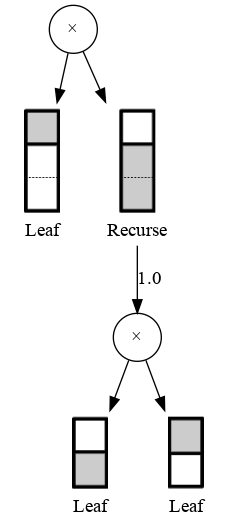
\includegraphics[scale=0.3]{graphs/cc1.png}
    \caption{\label{fig:basey-1}}
  \end{subfigure}
  \begin{subfigure}[b]{0.3\linewidth}
    \centering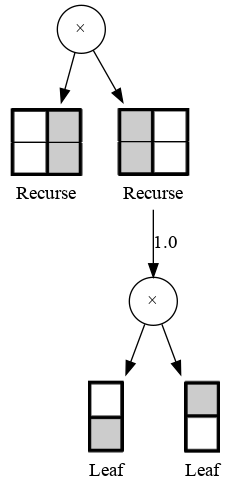
\includegraphics[scale=0.3]{graphs/cc4.png}
    \caption{\label{fig:basey-2}}
  \end{subfigure}
  \begin{subfigure}[b]{0.3\linewidth}
    \centering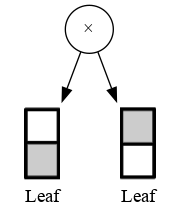
\includegraphics[scale=0.3]{graphs/cc5.png}
    \caption{\label{fig:basey-2}}
  \end{subfigure}
  \captionsetup{justification=raggedright}
  \caption{Special cases for the $y$-axis. Note how in both first cases the newly created sum node
  on the right has only one edge with weight $1$. This sum node is redundant and the SPN can be
  simplified by removing the sum node and adding its children as children of the parent product
  node. The far right case occurs when there are only two $k$ regions on the $y$-axis.}\label{fig:basey}
\end{figure}

These sub-SPNs showcase the three possible situations in which we may create a leaf node. Although
they refer to the $y$-axis, we can easily conclude the same for the $x$-axis, as
\autoref{fig:basex} illustrates. Note how in~\autoref{fig:basey-1} and~\autoref{fig:basey-2}, after
we recurse through the $1\times 2$ $k$-sized rectangles, we end up with a sum node that has only
one child. This creates a redundancy, as the value of the sum node would be the same as replacing
the sum node in question with its only child. We take this case into account in our algorithm,
watching for $2\times 1$ rectangles for the $x$-axis and $1\times 2$ rectangles for the $y$-axis.

\begin{figure}[h]
  \centering
  \begin{subfigure}[b]{0.3\linewidth}
    \centering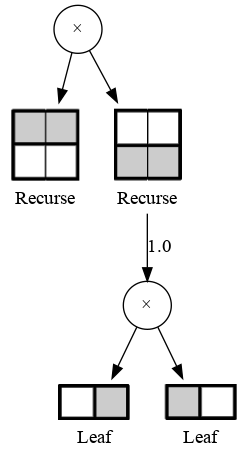
\includegraphics[scale=0.35]{graphs/cc2.png}
    \caption{\label{fig:basex-1}}
  \end{subfigure}
  \begin{subfigure}[b]{0.3\linewidth}
    \centering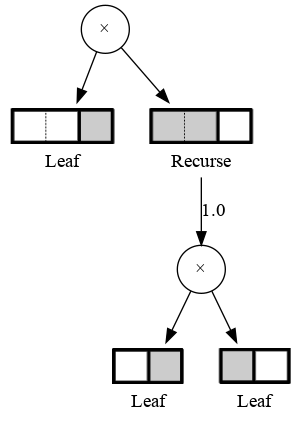
\includegraphics[scale=0.35]{graphs/cc3.png}
    \caption{\label{fig:basex-2}}
  \end{subfigure}
  \begin{subfigure}[b]{0.3\linewidth}
    \centering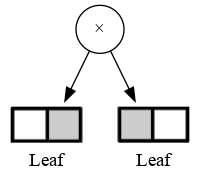
\includegraphics[scale=0.35]{graphs/cc6.png}
    \caption{\label{fig:basex-2}}
  \end{subfigure}
  \captionsetup{justification=raggedright}
  \caption{Special cases for the $x$-axis. Just like the $y$-axis, there is a redundant sum node
  with weight $1$ that can be removed and the SPN simplified in the two first cases. The third case
  illustrates the base case when there are only two $k$-sized rectangles placed horizontally.}\label{fig:basex}
\end{figure}

Now that we have our special base cases figured out, we can start building our algorithm. We will
divide our algorithm into two parts. In one we iterate through all possible $k$-resolution regions
that are $x$-aligned. For each of these regions, we check for the special cases mentioned above. If
none of those occur in our current region, then we recurse. In the other we do the same, but with
the $y$-axis. Each of these two parts should return two product nodes that can be interpreted as a
partitioning of the image into each axis regions. We then create a sum node and add the two
resulting product nodes as children. This sum node is the SPN of the image.

Note how this algorithm always creates two children for sum nodes and a decreasing number of
children for product nodes at each layer. Furthermore, the number of layers of the SPN is fixed
according to the size of the image. We also pre-initialized the weights of sum nodes to a uniform
distribution.

\begin{algorithm}[H]
  \caption{\mcode{GenerateDenseSPN$(k, p_0, p_1, \dset{D})$}}\label{alg:structure}
  \begin{algorithmic}[1]
    \Require\,Region resolution $k$
    \Require\,Top-left position $p_0= (x,y)$ of the underlying image area
    \Require\,Bottom-right position $p_1= (x,y)$ of the underlying image area
    \Require\,Dataset $\dset{D}$ containing instances of variable set $\mathbf{X}$
    \Ensure\,A dense SPN structure created from dataset $\dset{D}$
    \State\,n $\gets$ $\lceil\frac{p_1.x-p_0.x}{k}\rceil$
    \State\,m $\gets$ $\lceil\frac{p_1.y-p_0.y}{k}\rceil$
    \State\,$S$ $\gets$ \mcode{NewSum$()$}
    \State\,$q \gets (p_0.x, p_1.y)$
    \If{$n>1$}
      \For{$i\gets 1$ to $n$}
        \State\,$q \gets (\min\{p_1.x, q.x + k\}, p_1.y)$
        \State\,$r \gets (q.x, p_0.y)$
        \State\,$\Pi \gets$ \mcode{NewProduct$()$}
        \State\,Let $c_1$ and $c_2$ be children of $\Pi$
        \State\,$a_1 \gets$ \mcode{Area$(p_0, q, k)$}
        \State\,$a_2 \gets$ \mcode{Area$(r, p_1, k)$}
        \If{$a_1 = 1$}
          \State\,$c_1 \gets$ \mcode{NewLeaf$(p_0, q, \dset{D})$}
        \ElsIf{$a_1 = 2$}
          \State\,$c_1 \gets$ \mcode{NewProduct$()$}
          \State\,$\hat{c}_1 \gets$ \mcode{NewLeaf$(p_0, p_0+(k, k), \dset{D})$}
          \State\,$\hat{c}_2 \gets$ \mcode{NewLeaf$(p_0+(k, 0), q, \dset{D})$}
          \State\,\mcode{$c_1$.AddChildren$(\hat{c}_1, \hat{c}_2)$}
        \Else%
          \State\,$c_1 \gets$ \mcode{GenerateDenseSPN$(k, p_0, q, \dset{D})$}
        \EndIf%
        \State\,\mcode{$\Pi$.AddChild$(c_1)$}
        \If{$a_2 = 1$}
          \State\,$c_2 \gets$ \mcode{NewLeaf$(r, p_1, \dset{D})$}
        \ElsIf{$a_2 = 2$}
          \State\,$c_2 \gets$ \mcode{NewProduct$()$}
          \State\,$\hat{c}_1 \gets$ \mcode{NewLeaf$(r, r+(k, k), \dset{D})$}
          \State\,$\hat{c}_2 \gets$ \mcode{NewLeaf$(r+(k, 0), p_1, \dset{D})$}
          \State\,\mcode{$c_2$.AddChildren$(\hat{c}_1, \hat{c}_2)$}
        \Else%
          \State\,$c_2 \gets$ \mcode{GenerateDenseSPN$(k, r, p_1, \dset{D})$}
        \EndIf%
        \State\,\mcode{$\Pi$.AddChild$(c_2)$}
        \State\,\mcode{$S$.AddChild$(\Pi, 1/n)$}
      \EndFor%
    \EndIf%
    \algstore{alg:structure}
  \end{algorithmic}
\end{algorithm}

\begin{algorithm}[H]
  \caption*{\mcode{GenerateDenseSPN} (continued)}
  \begin{algorithmic}[1]
    \algrestore{alg:structure}
    \State\,$q \gets (p_1.x, p_0.y)$
    \If{$m > 1$}
      \For{$j \gets 1$ to $m$}
        \State\,$q \gets (p_1.x, \min\{p_1.y, q.y + k\})$
        \State\,$r \gets (p_0.x, q.y)$
        \State\,$\Pi \gets$ \mcode{NewProduct$()$}
        \State\,Let $c_1$ and $c_2$ be children of $\Pi$
        \State\,$a_1 \gets$ \mcode{Area$(p_0, q, k)$}
        \State\,$a_2 \gets$ \mcode{Area$(r, p_1, k)$}
        \If{$a_1 = 1$}
          \State\,$c_1 \gets$ \mcode{NewLeaf$(p_0, q, \dset{D})$}
        \ElsIf{$a_1 = 2$}
          \State\,$c_1 \gets$ \mcode{NewProduct$()$}
          \State\,$\hat{c}_1 \gets$ \mcode{NewLeaf$(p_0, p_0+(k, k), \dset{D})$}
          \State\,$\hat{c}_2 \gets$ \mcode{NewLeaf$(p_0+(0, k), q, \dset{D})$}
          \State\,\mcode{$c_1$.AddChildren$(\hat{c}_1, \hat{c}_2)$}
        \Else%
          \State\,$c_1 \gets$ \mcode{GenerateDenseSPN$(k, p_0, q, \dset{D})$}
        \EndIf%
        \State\,\mcode{$\Pi$.AddChild$(c_1)$}
        \If{$a_2 = 1$}
          \State\,$c_2 \gets$ \mcode{NewLeaf$(r, p_1, \dset{D})$}
        \ElsIf{$a_2 = 2$}
          \State\,$c_2 \gets$ \mcode{NewProduct$()$}
          \State\,$\hat{c}_1 \gets$ \mcode{NewLeaf$(r, r+(k, k), \dset{D})$}
          \State\,$\hat{c}_2 \gets$ \mcode{NewLeaf$(r+(0, k), p_1, \dset{D})$}
          \State\,\mcode{$c_2$.AddChildren$(\hat{c}_1, \hat{c}_2)$}
        \Else%
          \State\,$c_2 \gets$ \mcode{GenerateDenseSPN$(k, r, p_1, \dset{D})$}
        \EndIf%
        \State\,\mcode{$\Pi$.AddChild$(c_2)$}
        \State\,\mcode{$S$.AddChild$(\Pi, 1/m)$}
      \EndFor%
    \EndIf%
    \State\,\textbf{return} $S$
  \end{algorithmic}
\end{algorithm}

The actual code is available at \url{https://github.com/RenatoGeh/gospn}.

%--------------------------------------------------------------------------------------------------

\printbibliography[]

\end{document}
